%%%%%%%%%%%%%%%%%%%%%%%%%%%%%%%%%%%%%%%%%%%%%%%%%%%%%%%%%%%%%%%%%
% Contents : The reconciliation chapter
% $Id : grisbi-manuel-reconciliation.tex, v 0.4 2002/10/27 Daniel Cartron
% $Id : grisbi-manuel-reconciliation.tex, v 0.5.0 2004/06/01 Loic Breilloux
% $Id : grisbi-manuel-reconciliation.tex, v 0.6.0 2011/11/17 Jean-Luc Duflot
% $Id : grisbi-manuel-reconciliation.tex, v 0.8.9 2012/04/27 Jean-Luc Duflot
% $Id : grisbi-manuel-reconciliation.tex, v 1.0 2014/02/12 Jean-Luc Duflot
%%%%%%%%%%%%%%%%%%%%%%%%%%%%%%%%%%%%%%%%%%%%%%%%%%%%%%%%%%%%%%%%%

\chapter{Rapprochement bancaire\label{reconciliation}}


Les rapprochements bancaires servent à vérifier la bonne correspondance entre l'historique des opérations dans votre compte bancaire et les opérations saisies dans Grisbi. Faire un rapprochement bancaire consiste donc à faire une comparaison entre un relevé de votre compte  bancaire et les opérations enregistrées dans le compte correspondant dans Grisbi. Un rapprochement dans Grisbi est une représentation d'un relevé bancaire, comprenant un solde initial, des opérations et un solde final. Cette représentation est figée, comme le relevé bancaire. Donc une fois qu'un rapprochement est terminé et est correct, on ne devrait pas avoir à le modifier, sauf dans des cas exceptionnels.

Il est conseillé de faire les rapprochements de vos comptes régulièrement : cela permet aussi de détecter, autant dans Grisbi que dans votre relevé bancaire, des oublis ou des erreurs de saisie d'opérations, des décalages de tirage d'opérations, l'existence de frais bancaires, etc.


\section{Rapprochement d'un compte\label{reconciliation-account}}


Pour faire un rapprochement bancaire, munissez-vous du relevé de votre compte bancaire, et affichez la liste des opérations du compte correspondant sur Grisbi (voir le chapitre \vref{transactions}, \menu{Opérations d'un compte}).


\subsection{Description\label{reconciliation-account-description}}

Pour avoir accès à la fonction de rapprochement bancaire, cliquez sur \menu{Rapprocher} dans la barre \ifIllustration d'outils\refimage{reconciliation-list-img}.
\else d'outils.
\fi

\ifIllustration
% image centrée
\begin{figure}[htbp]
\begin{center}
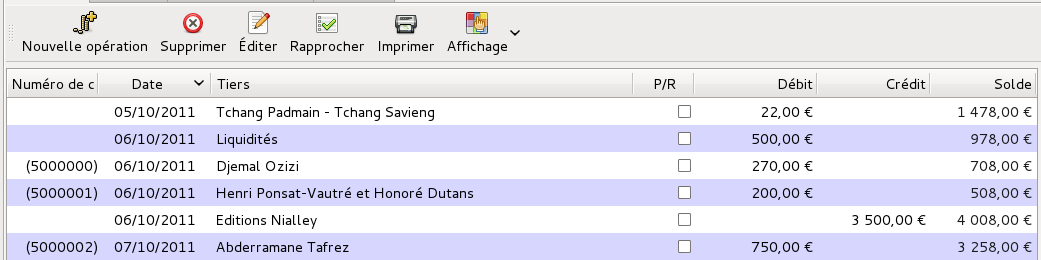
\includegraphics[scale=0.5]{image/screenshot/reconciliation_list}
\end{center}
\caption{Liste des opérations pendant un rapprochement}
\label{reconciliation-list-img}
\end{figure}
% image centrée
\fi

Les opérations s'affichent alors en mode \menu{Vue simple} (une seule ligne)\ifIllustration \refimage{reconciliation-list-img}, et la zone de rapprochement apparaît à gauche, en-dessous du panneau de navigation.
\else , et la zone de rapprochement apparaît à gauche, en-dessous du panneau de navigation.
\fi

L'affichage et le fonctionnement de la liste d'opérations se comportent de la même manière qu'en dehors de la fonction de rapprochement, en résumé : largeur et libellé des colonnes, déplacement de la liste, \indexword{affichage des opérations}\index{affichage !opérations}, menu contextuel, affichage des champs, \indexword{\glspl{tri}} des opérations\index{tri !opérations}.

Vous pouvez donc exécuter sur cette liste les mêmes actions qu'en dehors de la fonction de rapprochement, que ce soit au moyen de la barre d'outils ou du menu contextuel : sélection, création, ventilation, modification, suppression, etc. Reportez vous pour cela au chapitre \vref{transactions}, \menu{Opérations d'un compte}.

%espace pour changement de thème
\vspacepdf{5mm}

La zone de rapprochement comporte plusieurs éléments :
% espace avant image 5mm
\vspacepdf{3mm}

% Pas de référence à l'illustration car erreur de numéro de figure avec picins.
\begin{itemize}
	\ifIllustration
	% image entourée par une liste (picins)
	% supprimé car en html les figures entourées ne sont pas numérotées, et la numérotation des figures centrées décalée par rapport au pdf
	%\piccaption{Zone de rapprochement}
	\label{reconciliation-infos-img}
	\parpic[r]{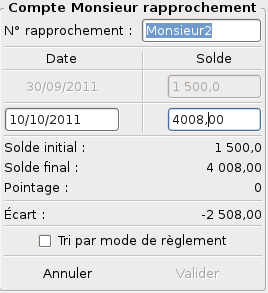
\includegraphics[scale=0.5]{image/screenshot/reconciliation_infos}}
	% image entourée par une liste (picins)
	\fi
	 \item le nom du compte à rapprocher, suivi de \og rapprochement \fg{} ;
	 \item une zone de saisie \menu{\No rapprochement} pour le numéro de rapprochement ;
	 \item un tableau de deux colonnes pour les dates et les soldes, et de deux lignes pour le rapprochement précédent et celui en cours ; seule la deuxième ligne est constituée de champs de saisie ; 
	 \item trois lignes pour le \indexword{solde initial}\index{solde !initial}, le \indexword{solde final}\index{solde !final} et le \indexword{pointage}\index{pointage}, qui est la somme des opérations pointées ;
	 \item une ligne pour l'écart, qui est différent de zéro tant que le total des pointages ne correspond pas à la différence entre le solde initial et le solde final du relevé bancaire ;
	 \item une ligne pour le choix du \gls{tri} par mode de règlement ;
	 \item les boutons \menu{Annuler} et \menu{Valider}.
\end{itemize}

% espace pour changement de thème
\vspacepdf{5mm}

Le \menu{\No rapprochement} est le seul paramètre qui permet d'identifier à coup sûr un rapprochement quelconque ; ce numéro peut comprendre du texte et des nombres. Par défaut, Grisbi attribue un numéro à chaque rapprochement, composé du nom du compte concerné, suivi d'un nombre ; ce nombre est incrémenté automatiquement au rapprochement suivant. Ce \menu{\No rapprochement} est donc unique pour chaque rapprochement d'un compte, et il est visible dans le menu \menu{Préférences - Rapprochement} (voir la section \vref{setup-operations-reconciliation}, \menu{Rapprochement}. 

Grisbi vous permet de personnaliser cette numérotation, qui devra être de la forme \og texte + nombre \fg{}, pour être unique pour chacun de vos rapprochements. Vous pouvez inventer la numérotation qui vous convient, et ce, compte par compte ; par exemple, ils pourront porter le même numéro que vos relevés bancaires. Si, pour quelque raison, le \menu{\No rapprochement} ne respecte pas cette forme, il vous sera difficile de retrouver son contenu, c'est à dire les opérations qui lui appartiennent (voir la section \vref{reconciliation-manage-content}, \menu{Contenu d'un rapprochement}) ; cependant, vous pourrez toujours y modifier le numéro de chaque rapprochement, mais cela risque d'être assez fastidieux \ldots

% espace avant Attention ou Note  : 5 mm
\vspacepdf{5mm}
\textbf{Note} : s'il vous est possible d'avoir la même \indexword{numérotation}\index{rapprochement !numérotation} pour les rapprochements (par ex. de 1 à n) dans des comptes différents, il est impossible de l'avoir plusieurs fois dans un même compte. Vous pourrez par exemple prévoir une numérotation du type année-numéro : 2003-01 pour votre premier relevé mensuel de 2003, et ensuite Grisbi numérotera les suivants jusqu'à 2003-12 ; l'année suivante vous numéroterez le premier 2004-01, etc. Quelque soit le contenu de votre numérotation, il suffit que la fin soit numérique pour que Grisbi sache l'incrémenter, par exemple AV-001 ou REM-001, ou bien encore CCP-1106 pour compte CCP année 2011 mois 06, qui ne permettra aucune confusion sur les comptes et les dates. 
% espace après Attention ou Note  : 5 mm
\vspacepdf{5mm}

Les date et solde du \indexword{rapprochement précédent}\index{rapprochement !précédent} sont automatiquement repris du dernier rapprochement, donc ne sont pas modifiables, et sont en grisé. Mais ce ne sera bien évidemment pas le cas lors du premier rapprochement, où le solde initial est celui que vous avez entré lors de la création du compte (voir la section \vref{accounts-properties}, \menu{Propriétés d'un compte}).

La date du \indexword{rapprochement en cours}\index{rapprochement !en cours} peut être saisie avec le clavier ou le calendrier, disponibles comme dans tout champ de date dans Grisbi (voir les sections \vref{transactions-new-dates}, \menu{Saisie de date au clavier} ou \vref{transactions-new-calendar}, \menu{Saisie de date au calendrier}).

% espace avant Attention ou Note  : 5 mm
\vspacepdf{5mm}
\strong{Attention} : la date finale du rapprochement précédent et la date initiale du rapprochement en cours peuvent être identiques, ou doivent se suivre chronologiquement, pour ne pas avoir de chevauchement de périodes de rapprochement ; cependant, si vous avez fait de telles erreurs, Grisbi pourra probablement les corriger : voir la section \vref{reconciliation-manage}, \menu {Gestion des rapprochements des comptes}.
% espace arès Attention ou Note  : 5 mm
\vspacepdf{5mm}

Afin de faciliter l'identification des opérations pendant le rapprochement vous pouvez toujours changer l'\indexword{ordre d'affichage} des opérations\index{rapprochement !ordre d'affichage}, pour qu'il corresponde à celui de votre relevé bancaire. Ou bien, si vous avez beaucoup d'opérations à rapprocher, vous pouvez par exemple les classer par ordre de montants croissants ou décroissants, pour faciliter la recherche d'un montant ; quand le rapprochement sera terminé, vous rétablirez le classement par date pour avoir un solde juste en fin de liste (voir la section \vref{transactions-list-sorts}, \menu{Tris}).

% espace pour changement de thème : 5 mm
\vspacepdf{5mm}
Vous pouvez aussi trier les opérations en cochant la case \menu{Tri par mode de règlement} dans la zone de rapprochement, ou bien en configurant l'ordre d'affichage selon ces modes de règlement, individuellement pour chaque compte, dans le menu  \menu{Édition - Préférences} (voir la section \vref{setup-operations-sort}, \menu{Option de tri pour les rapprochements}).

% espace pour changement de thème : 5 mm
\vspacepdf{5mm}
Vous pouvez encore masquer ou afficher les \indexword{opérations rapprochées}\index{affichage  !opérations rapprochées} (\og \textbf{R} \fg{}), grâce aux choix proposés par la fonction \menu{Affichage} de la barre de menus ou de la barre d'outils, ou bien, plus simplement, par la combinaison de touches \key{Alt}\key{R}. 

\subsection{Procédure de rapprochement\label{reconciliation-account-howto} }

La procédure pour opérer un rapprochement est la suivante :

\begin{enumerate}
	 \item dans la barre d'outils, cliquez sur \menu{Rapprocher} ;
	 \item vérifiez que la \indexword{zone de rapprochement}\index{rapprochement !zone} affiche un \indexword{numéro de rapprochement}\index{rapprochement !numéro}, sinon saisissez-en un, sous la forme \og texte + nombre \fg{} qui sera unique pour chacun d'eux ; pour les rapprochements suivants, Grisbi incrémentera automatiquement ce nombre ;
	 % saut de ligne pour indentation correcte de la note dans la liste
 
\textbf{Note} : l'incrémentation ne fonctionnera que si la numérotation de votre rapprochement se termine par un chiffre, par exemple \og CCP-201106 \fg{}, et pas du tout dans le cas de \og 201106-CCP \fg{}.
		
	 \item la première ligne du tableau indique la date du rapprochement précédent et le solde à cette date, qui sont alors la date et le solde initiaux de votre rapprochement en cours : ils sont en grisé, vous ne pouvez donc pas les modifier ; ce solde initial est aussi celui de votre dernier relevé bancaire ; il est reporté dans la ligne \menu{\indexword{Solde initial}}\index{solde ! initial} en-dessous ;
	 \item dans la seconde ligne du tableau, saisissez la date du jour (ou celle du relevé bancaire) (voir les sections \vref{transactions-new-dates}, \menu{Saisie de date au clavier} ou \vref{transactions-new-calendar}, \menu{Saisie de date au calendrier}) ainsi que le solde courant, que vous trouvez sur votre dernier relevé bancaire : ce sont la date et le solde de fin de votre rapprochement ; de même, ce solde est reporté dans la ligne \menu{Solde final} en-dessous ;
	 \item dans la liste des opérations, pour chaque opération commune à votre compte et votre relevé bancaires, cochez l'opération dans votre relevé bancaire, et pointez dans Grisbi l'opération par l'un des moyens suivants :
	 
		\begin{itemize}
			\item cliquez sur la ligne d'opération dans la \indexword{colonne} \menu{P/R}\index{colonne !P/R},
			\item appuyez sur la  combinaison de touches \key{Ctrl}\key{P},
			\item appuyez sur la barre d'espace (ce qui déplace aussi la sélection sur la ligne en-dessous) ;			
		\end{itemize}	 
un \og \textbf{P} \fg{} y apparaît alors pour indiquer que l'opération est \og pointée \fg{} ; si vous vous êtes trompé(e), un autre clic, un autre \key{Ctrl}\key{P} ou un autre appui sur la barre d'espace (précédé du déplacement de la sélection sur la ligne au-dessus) supprime le \og \textbf{P} \fg{} ; à chaque nouveau \og \textbf{P} \fg{}, dans la colonne \menu{P/R}, la ligne \menu{Pointage} de la zone de rapprochement est augmentée du même montant, en positif si c'est un crédit et en négatif si c'est un débit, et la ligne \menu{Écart} fait de même ;
	 \item lorsque vous avez coché toutes les opérations de votre relevé bancaire, et toutes celles correspondantes dans la liste d'opérations de Grisbi, la ligne 	\menu{Écart} doit indiquer zéro et la ligne \menu{Pointage} doit indiquer la même valeur que la différence entre la ligne \menu{Solde initial} et la ligne \menu{Solde final} ; si ce n'est pas le cas, c'est qu'il s'est glissé une erreur quelque part dans une opération, dans un solde ou ailleurs ;
	 \item si vous voulez interrompre le \indexword{rapprochement}\index{rapprochement !interrompre} en cours, invalidez par le bouton \menu{Annuler} : Grisbi supprime la zone de rapprochement, mais les opérations pointées dans la liste le restent ; ainsi, lorsque vous reprendrez le rapprochement, les pointages ne seront pas perdus ; par contre, il vous faudra saisir à nouveau la date et le solde ;
	 \item quand tout est correct dans la zone de rapprochement, en particulier quand le contenu de \menu{Écart} est nul, le bouton \menu{Valider} devient opérationnel, alors cliquez dessus ; Grisbi supprime la zone de rapprochement, et remplace les \og \textbf{P} \fg{} par des \og \textbf{R} \fg{} dans la liste des opérations, pour indiquer que ces opérations-là sont \og rapprochées \fg{} ; à partir de ce moment, ces opérations ne sont plus que partiellement modifiables, car les montants sont figés (puisque c'est leur exactitude et leur correspondance avec le relevé bancaire qui sont le but même de l'opération de rapprochement).
\end{enumerate}

Après un rapprochement, si vous voulez ne plus afficher les \indexword{opérations rapprochées}\index{affichage !opérations rapprochées} (\og \textbf{R} \fg{}) dans la liste des opérations, sélectionnez, dans la barre de menus ou dans la barre d'outils, la fonction \menu{Affichage - Montrer les opérations rapprochées}, ou bien, plus simplement, appuyez sur la combinaison de touches \key{Alt}\key{R}. La même action réaffiche les opérations rapprochées.

% espace avant Attention ou Note  : 5 mm
\vspacepdf{5mm}
\textbf{Note} : si vous annulez un rapprochement avant de l'avoir complètement terminé et validé, la liste d'opérations affichera comme \og \indexword{pointées}\index{opération !pointée} \fg{} les opérations qui l'ont été pendant le rapprochement interrompu. Cela permet de reprendre le rapprochement ultérieurement. Vous pouvez cependant \og dé-pointer \fg{} chacune de ces opérations par la combinaison de touches \key{Ctrl}\key{P}.

% espace avant Attention ou Note  : 5 mm
\vspacepdf{5mm}
\textbf{Note} : pour que la recherche d'erreurs éventuelles ne soit pas trop difficile, il est recommandé de faire le rapprochement bancaire régulièrement, si possible à chaque réception de relevé de banque, et de toutes façons quand il n'y a pas trop d'opérations non pointées.


\section{Gestion des rapprochements des comptes\label{reconciliation-manage}}


\subsection{Gestion des paramètres des rapprochements\label{reconciliation-manage-parameters}}

Pour gérer les \indexword{paramètres des rapprochements}\index{rapprochement !paramètres}, vous disposez des fonctionnalités suivantes :

\begin{itemize}
	\item lister tous les rapprochements réalisés sur tous les comptes ;
	\item supprimer des rapprochements ;
	\item afficher les détails de chacun d'eux ;
	\item vérifier la cohérence des dates de rapprochement (successives, sans recouvrement de périodes).
\end{itemize}

% espace pour changement de thème  : 5 mm
\vspacepdf{5mm}
Un assistant permet aussi d'aider à rétablir la continuité des rapprochements et de réparer certaines erreurs.

Ces fonctionnalités sont disponibles dans le menu \menu{Édition - Préférences}, et sont décrites en détail dans la section \vref{setup-operations-reconciliation}, \menu{Rapprochement}.


\subsection{Contenu d'un rapprochement\label{reconciliation-manage-content}}

Vous ne pouvez afficher le \indexword{contenu d'un rapprochement}\index{rapprochement !contenu} que s'il dispose d'un \menu{\No rapprochement} unique. Si ce n'est pas le cas, vous devrez d'abord modifier le \menu{\No rapprochement} pour chacun des rapprochements du compte, avec un numéro de la forme \og texte + nombre \fg{}, le nombre s'incrémentant à chaque rapprochement suivant (voir la section \vref{setup-operations-reconciliation}, \menu{Rapprochement}). Si c'est déjà le cas, vous pouvez utiliser l'une de ces deux méthodes :

\begin{itemize}
	\item dans la liste des opérations, trier les opérations suivant le critère \menu{\No rapprochement} : c'est la méthode la plus rapide ;
	\item créer un état des opérations appartenant à un \menu{\No rapprochement} connu :  cette méthode permet d'en mémoriser son contenu.
\end{itemize}


\subsubsection{Tri des opérations par \menu{\No rapprochement}\label{reconciliation-manage-content-sort}}

Pour afficher les opérations d'un compte suivant un tel tri, procédez comme suit :

\begin{enumerate}
	\item affichez le champ \menu{\No rapprochement} dans les cellules de la liste des opérations : deux méthodes existent :
		\begin{itemize}
			\item configurez l'affichage des cellules de la liste des opérations dans le menu \menu{Édition - Préférences} : voir le paragraphe \menu{Contenu de la liste des opérations} (section \vref{setup-operations-cells}, \menu{Cellules de la liste des opérations}),
			\item dans la liste des opérations, sélectionnez le nombre de lignes nécessaires pour afficher le champ \menu{\No rapprochement}, puis modifiez l'affichage de la liste des opérations : voir la section \vref{transactions-list-fields-manage}, \menu{Gestion des champs d'information} ;	 
		\end{itemize}			 	
	\item dans la liste des opérations, sélectionnez le nombre de lignes nécessaires pour afficher le champ \menu{\No rapprochement}, puis sélectionnez ce critère de tri dans la colonne contenant ce champ (voir la section \vref{transactions-list-sorts}, \menu{Tris}).
\end{enumerate}


\subsubsection{État des opérations appartenant à un \menu{\No rapprochement} connu\label{reconciliation-manage-content-report}}

Pour créer un état des opérations appartenant à un \menu{\No rapprochement} connu, procédez comme suit :

\begin{enumerate}
	\item sélectionnez l'onglet \menu{États}, puis choisissez \menu{Recherche} dans la liste déroulante ; 
	\item faites les choix adaptés à votre recherche dans les différents onglets, notamment :
		\begin{itemize}
			\item dans l'onglet \menu{Textes}, cochez \menu{Sélectionnez les opérations d'après leur contenu}, choisissez \menu{\No rapprochement} dans la liste déroulante de libellé \menu{Opérations dont}, puis saisissez le numéro de rapprochement recherché dans le champ de libellé \menu{contient} ;
			\item dans l'onglet \menu{Généralités}, saisissez un nom dans le champ \menu{Nom de l'état} ;
			\item dans l'onglet \menu{Opérations}, cochez au moins \menu{Afficher les opérations}, \menu{tiers}, \menu{date}, \menu{\No rapprochement}, \menu{Afficher les titres des colonnes}	 ;
		\end{itemize}	
	
	\item validez la fenêtre : la liste des opérations appartenant au rapprochement recherché s'affiche.
\end{enumerate}

% espace pour changement de thème  : 5 mm
\vspacepdf{5mm}
Vous pouvez toujours modifier ensuite vos sélections en cliquant sur l'outil \menu{Propriétés} dans la barre d'outils (voir aussi le chapitre \vref{reportscreation}, \menu{Création d'un état}).


\section{Résolution de problèmes de rapprochement\label{reconciliation-solve}}


Il se peut que vous n'arriviez pas à faire votre \indexword{rapprochement}\index{rapprochement !problèmes} correctement. Cela peut être dû à des erreurs de pointage, de saisie d'opération, ou même d'erreurs dans votre relevé de compte bancaire. Ces erreurs sont généralement facilement identifiées en reprenant avec attention le pointage des opérations, tant sur Grisbi que sur votre relevé de compte. C'est aussi pour cela que les rapprochements doivent être faits régulièrement, ou tout au moins tant que le nombre d'opérations à pointer ne dépasse pas quelques dizaines.

% espace avant Attention ou Note  : 5 mm
\vspacepdf{5mm}
\textbf{Note} : pour tous les cas décrits dans les sections suivantes, commencez par faire un test de débogage de votre fichier de comptes, qui vous permettra de préciser où se trouvent d'éventuels problèmes (voir la section \vref{maintenance-file-debug}, \menu{Déboguer le fichier de comptes}).


\subsection{Rapprochement sur un compte nouveau\label{reconciliation-solve-new}}

Si vous utilisez Grisbi depuis un certain temps, et que vous ouvrez un nouveau compte bancaire à la banque, comme le solde de ce compte est nul, vous créez un nouveau compte dans Grisbi avec un solde initial nul ; vous saisirez le premier versement sur le compte bancaire par une opération initiale dans le nouveau compte dans Grisbi. C'est le cas le plus simple, qui ne pose de problème pour aucun rapprochement ultérieur.


\subsection{Rapprochement sur un compte ancien\label{reconciliation-solve-old}}

Par contre, si vous avez un compte bancaire depuis longtemps et que vous commencez à  utiliser Grisbi, vous créerez un compte dans Grisbi, soit en mettant un solde initial égal au solde du compte bancaire à ce jour, dans l'onglet \menu{Propriétés} du compte, soit en créant une opération de dépôt initial du même montant dans la liste des opérations du compte. 

% espace pour changement de thème  : 5 mm
\vspacepdf{5mm}
De ce fait, si vous voulez par la suite, pour avoir toutes vos opérations dans Grisbi, entrer des opérations antérieures à la date de première utilisation de Grisbi, vous devrez soit modifier le solde initial du compte, soit modifier l'opération de dépôt initial, du montant total de ces opérations antérieures. Dans ces deux cas, le solde des opérations dans la liste des opérations sera modifié automatiquement et sera correct, mais le solde initial de votre premier rapprochement, indiqué dans l'onglet \menu{Rapprochement} du menu \menu{Édition - Préférences}, ne sera pas modifié et sera donc incorrect ; ce qui fait que le rapprochement incluant ces opérations ne pourra pas être bon. De plus ces opérations ne seront associées à aucun rapprochement. Dans l'un et l'autre cas, voici comment résoudre cela :

% espace avant Attention ou Note  : 5 mm
\vspacepdf{5mm}
\strong{Attention} : il est fortement recommandé de faire une sauvegarde de votre fichier de comptes avant de faire les manipulations suivantes sur les rapprochements, car certaines erreurs pourraient rendre ce fichier inutilisable.

% espace après Attention ou Note  : 5 mm
\vspacepdf{5mm}

Si vous procédez en modifiant le solde initial du compte : 

\begin{enumerate}
	\item vérifiez que le dernier rapprochement de ce compte est fait et correct ;
	\item saisissez les opérations antérieures au premier rapprochement de ce compte ;	
	\item modifiez le solde initial du premier rapprochement dans l'onglet \menu{Rapprochement}, du montant total des opérations antérieures que vous venez de saisir ;
	\item modifiez la date initiale du premier rapprochement, pour une date antérieure à la date de l'opération la plus ancienne que vous avez ajoutée ;
	\item forcez en \menu{Rapproché} le statut de chaque opération antérieure ajoutée par un \key{Ctrl}\key{R} : une fenêtre s'ouvre, sélectionnez le premier rapprochement (celui dont vous avez changé la date initiale) pour associer ce rapprochement à l'opération, puis validez ; 
	\item  procédez éventuellement à une vérification des rapprochements par la fonction \menu{Trouver les opérations marquées et non associées à un rapprochement} dans l'onglet \menu{Rapprochement} du menu \menu{Édition - Préférences}.
\end{enumerate}

% espace pour séparation de la procédure : 5 mm
\vspacepdf{5mm}
Si vous procédez en modifiant l'opération de dépôt initial :
\begin{enumerate}
	\item vérifiez que le dernier rapprochement de ce compte est fait et correct ;
	\item saisissez les opérations antérieures au premier rapprochement de ce compte ;	
	\item modifiez le solde initial du premier rapprochement dans l'onglet \menu{Rapprochement}, du montant total des opérations antérieures que vous venez de saisir ;
	\item modifiez la date initiale du premier rapprochement, pour une date antérieure à la date de l'opération la plus ancienne que vous avez ajoutée ;
	\item changez le statut de l'opération de dépôt initial en \menu{ Non Rapproché} par un \key{Ctrl}\key{R} (pour pouvoir la modifier) ;
	\item modifiez le montant de cette opération du montant total des opérations antérieures que vous venez de saisir ;	
	\item forcez en \menu{Rapproché} le statut de l'opération de dépôt initial et de chaque opération antérieure ajoutée, par un \key{Ctrl}\key{R} : une fenêtre s'ouvre, sélectionnez le premier rapprochement (celui dont vous avez changé la date initiale) pour associer ce rapprochement à l'opération, puis validez ; 
	\item  procédez éventuellement à une vérification des rapprochements par la fonction de libellé \menu{Trouver les opérations marquées et non associées à un rapprochement} dans l'onglet \menu{Rapprochement} du menu \menu{Édition - Préférences}.
\end{enumerate}

% espace pour séparation de la procédure : 5 mm
\vspacepdf{5mm}
Vous aurez alors une liste d'opérations avec un solde correct, tous les rapprochements seront corrects et toutes les opérations saisies ou modifiées seront associées à un rapprochement.


